%ARCHITETTURA PLUG-IN
\section{Architettura del prodotto}
Il nostro prodotto\glosp è composto da un plug-in sviluppato per la piattaforma Grafana\glosp e un'applicazione ausiliaria, esterna a tale piattaforma. Perciò l'analisi dell'architettura è suddivisa in queste due componenti.
\subsection{Plug-in}
Per poter visualizzare la suddivisione delle componenti del plug-in e le dipendenze che sussistono tra loro ad alto livello, viene riportato il diagramma dei Package in allegato nel file \textit{diagramma-package-plug-in.png}.
\subsubsection{Progettazione architetturale}
Abbiamo deciso di utilizzare un design pattern\glosp architetturale Model-View-Controller (MVC) perché si adatta bene allo sviluppo software all'interno di Grafana\glo. In particolare, come si può vedere nella figura seguente, abbiamo la View che scambia informazioni sulle interazioni dell'utente con il Controller che a sua volta le trasforma in azioni sui dati eseguite da Model. Infine vi è una comunicazione tra Model e View per il costante aggiornamento di quest'ultima, grazie ad una funzionalità fornita dalla piattaforma Grafana\glo.
\mbox{}
\begin{landscape}
	\begin{figure}
		\begin{figure} [H]
			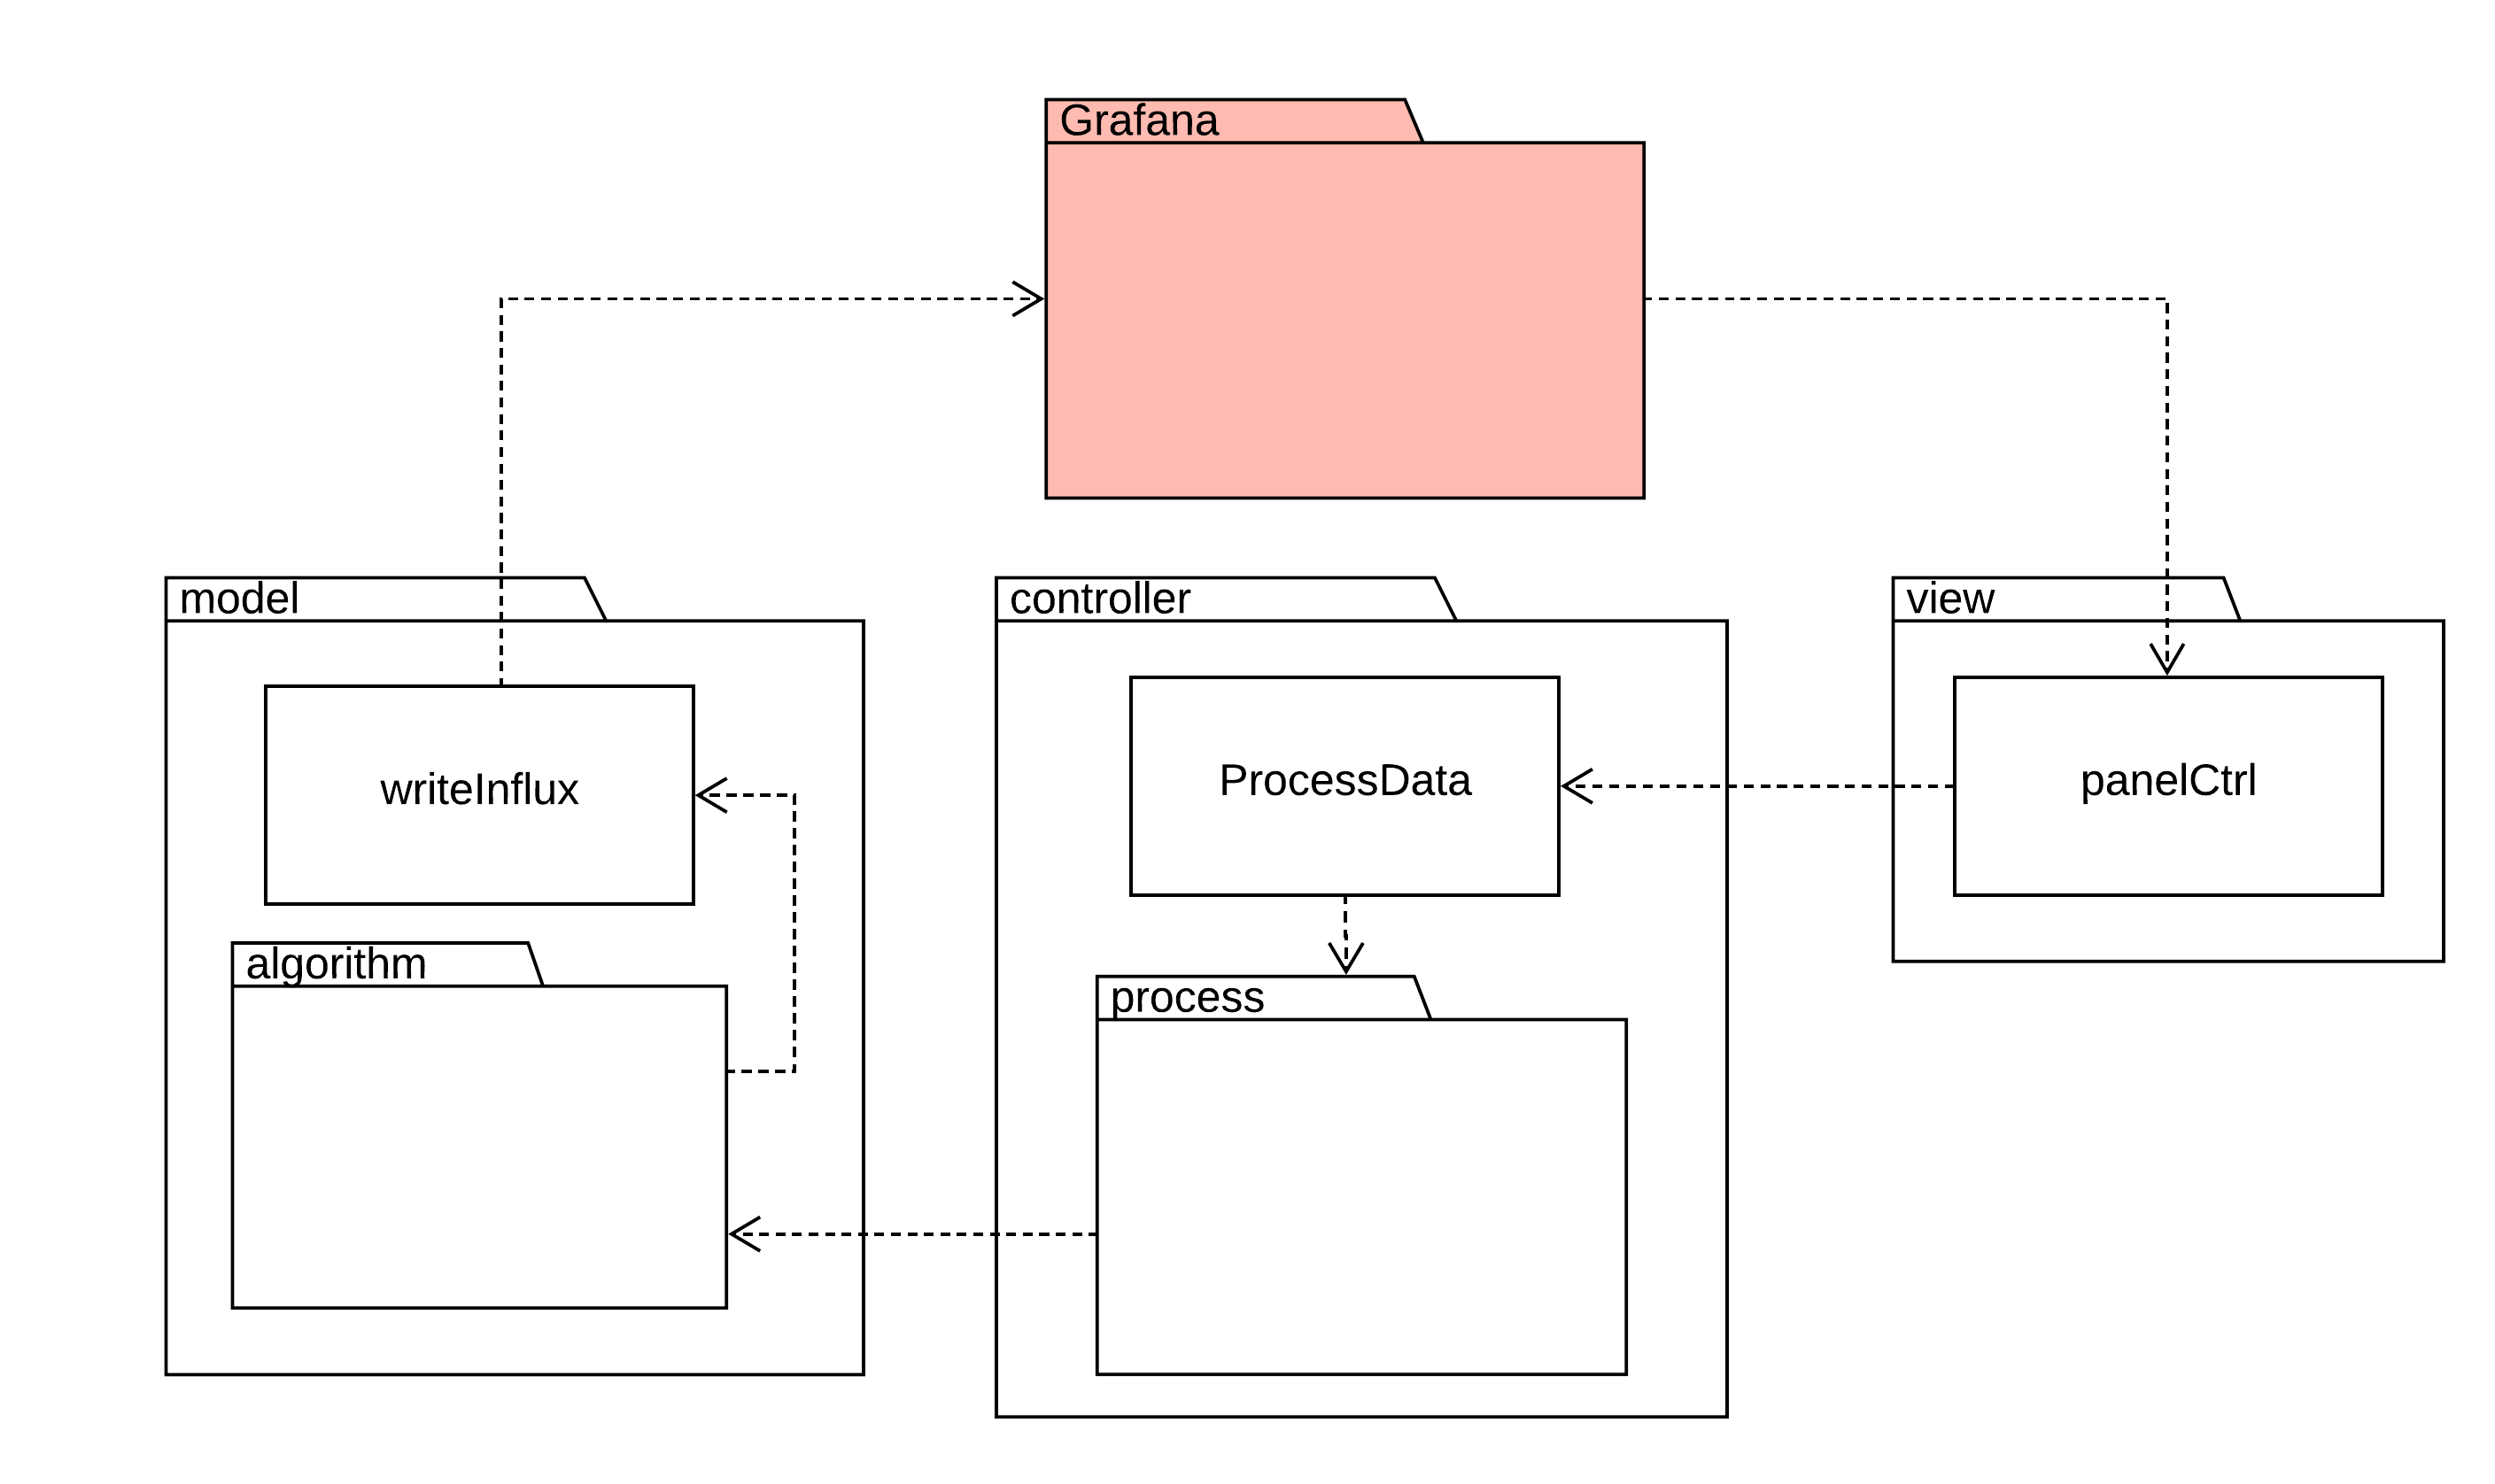
\includegraphics[width=\linewidth]{./img/Diagrammi/architettura-plug-in.png}
			\caption{Diagramma dell'architettura del plug-in}
		\end{figure}
	\end{figure}
\end{landscape}
Analizzando i componenti, la nostra architettura è così strutturata: 
\begin{itemize}
	\item \textbf{Model}: modulo che gestisce la business logic\glo. Più in dettaglio, contiene gli algoritmi di predizione dei dati che sono stati attualmente implementati e la scrittura del risultato delle predizioni su un database Influx;
	\item \textbf{View}: modulo che gestisce la presentation logic. Più in dettaglio, permette la creazione di un pannello grafico personalizzato all'interno di una dashboard Grafana\glo. Con questo pannello l'utente può selezionare le impostazioni degli algoritmi di predizione, i flussi di dati in ingresso, le impostazioni del grafico presente nel pannello e le impostazioni del database Influx su cui scrivere i risultati;
	\item \textbf{Controller}: modulo che gestisce l'application logic. Più in dettaglio, trasforma i dati ottenuti dalle interazioni dell'utente ed i flussi dati ottenuti da Grafana\glosp in un formato adatto per l'esecuzione delle azioni da parte del Model.
\end{itemize}
\paragraph{Ruolo di Grafana nell'architettura} \mbox{}\\ [1mm]
Grafana\glosp ricopre un ruolo fondamentale nell'architettura, infatti la sua presenza permette l'aggiornamento continuo della vista alla variazione dei dati nel modello. In particolare, ogni volta che sono presenti aggiornamenti sui dati nel modello, Grafana\glosp li rende disponibili alla vista tramite appositi metodi, assieme alla configurazione delle query con cui questi dati sono stati ottenuti. Inoltre, la sua presenza gestisce tramite AnuglarJS il two-way data binding tra vista HTML e codice Javascript, oltre che ad offrire la maggior parte dei componenti grafici necessari alla realizzazione della vista del plug-in.
\subsubsection{Progettazione di dettaglio}
Di seguito viene descritta in dettaglio la progettazione del plug-in. In allegato viene inoltre fornito il file \textit{diagramma-classi-plug-in.png} contenente l'intero diagramma delle classi.
\paragraph{Model} \mbox{}\\ [1mm]
Il componente principale del Model è l'interfaccia degli algoritmi di predizione chiamata \textit{AlgorithmPrediction}. A partire da questa, abbiamo implementato due algoritmi: Support Vector Machine\glosp lineare e Regressione lineare\glo. Essi sono rappresentati rispettivamente dalle classi concrete \textit{SvmPrediction} e \textit{RlPrediction}. In senso più generale, abbiamo riscontrato che, per famiglie di algoritmi Support Vector Machine\glosp e Regressione\glo, è possibile ricondursi ad un'interfaccia unica come abbiamo fornito.
La due classi concrete hanno inoltre una dipendenza di tipo composizione con un'altra classe concreta chiamata \textit{WriteInflux}. Essa permette di eseguire la scrittura su un database Influx attraverso due metodi che differiscono per il tipo di dati da salvare. Infine, importa la libreria \textit{InfluxDB} che utilizza per interfacciarsi con il database stesso.
\paragraph*{AlgorithmPrediction} \mbox{}\\ [1mm]
L'interfaccia degli algoritmi di predizione è chiamata \textit{AlgorithmPrediction} e rappresenta il contratto che tutte le classi concrete devono rispettare per poter caratterizzare un algoritmo di predizione. Essa contiene un solo metodo: \textit{predict(DataSet, Result, WriteInfluxParameters)}. Questo permette di eseguire la predizione su un determinato set di dati di tipo DataSet, con degli specifici parametri di configurazione di tipo Result e di scrittura nel database di tipo WriteInfluxParameters.
\paragraph*{SvmPrediction} \mbox{}\\ [1mm]
Per implementare l'algoritmo Support Vector Machine\glosp lineare abbiamo realizzato la classe concreta \textit{SvmPrediction}, implementando il metodo \textit{predict(DataSet, Result, WriteInfluxParameters)} dell'interfaccia \textit{AlgorithmPrediction}.
Questo metodo esegue la predizione sul set di dati e sulla base dei parametri di configurazione forniti in input. Inoltre fa uso di componenti specifici della classe SVM importata dalla libreria \textit{NodeModules} per effettuare la vera e propria previsione. \\
\textit{SvmPrediction} contiene inoltre due campi dati:
\begin{itemize}
	\item writeInflux: è un riferimento alla classe \textit{WriteInflux};
	\item predictor: è un riferimento alla classe \textit{SVM}.
\end{itemize}
Essi vengono istanziati solo al momento dell'utilizzo. \\
È infine presente il costruttore privo di parametri che permette di eseguire il binding dei metodi alla classe.
\paragraph*{RlPrediction} \mbox{}\\ [1mm]
Per implementare l'algoritmo Regressione lineare\glosp abbiamo realizzato la classe concreta \textit{RlPrediction}, implementando il metodo \textit{predict(DataSet, Result, WriteInfluxParameters)} dell'interfaccia \textit{AlgorithmPrediction}.
Questo metodo esegue la predizione sul set di dati e sulla base dei parametri di configurazione forniti in input. Inoltre fa uso della libreria \textit{LinearRegression}  che viene importata per effettuare la vera e propria previsione. \\
\textit{RlPrediction} contiene inoltre due campi dati:
\begin{itemize}
	\item writeInflux: è un riferimento alla classe \textit{WriteInflux};
	\item predictor: è un riferimento alla classe \textit{LinearRegression}.
\end{itemize}
Essi vengono istanziati solo al momento dell'utilizzo. \\
È infine presente il costruttore privo di parametri che permette di eseguire il binding dei metodi alla classe.
\paragraph*{WriteInflux} \mbox{}\\ [1mm]
Per interfacciarsi e scrivere i dati nel database Influx viene utilizzata la classe \textit{WriteInflux}. Essa viene instanziata all'interno del metodo \textit{predict(DataSet, Result, WriteInfluxParameters)} delle classi rappresentanti gli algoritmi di predizione. Contiene due campi dati:
\begin{itemize}
	\item influx: è un riferimento alla classe InfluxDB della libreria node-influx;
	\item parameters: è un riferimento al tipo WriteInfluxParameters e contiene i parametri per il collegamento e la scrittura nel database.
\end{itemize}
È presente il metodo costruttore che riceve in input un WriteInfluxParameters, ne esegue il setting ed instazia InfluxDB.
Infine sono presenti due metodi:
\begin{itemize}
	\item writeArrayToInflux(double[], long[]): esegue la scrittura di un array di dati, solitamente quelli predetti, usando come chiavi in InfluxDB i corrispondenti TimeStamps passati come parametro;
	\item writeStampsToInflux(double, long): esegue la scrittura di un singolo dato, solitamente predetto, usando come chiave in InfluxDB il suo relativo TimeStamps passato come parametro.
\end{itemize}
\mbox{}
\begin{landscape}
	\begin{figure}
		\begin{figure} [H]
			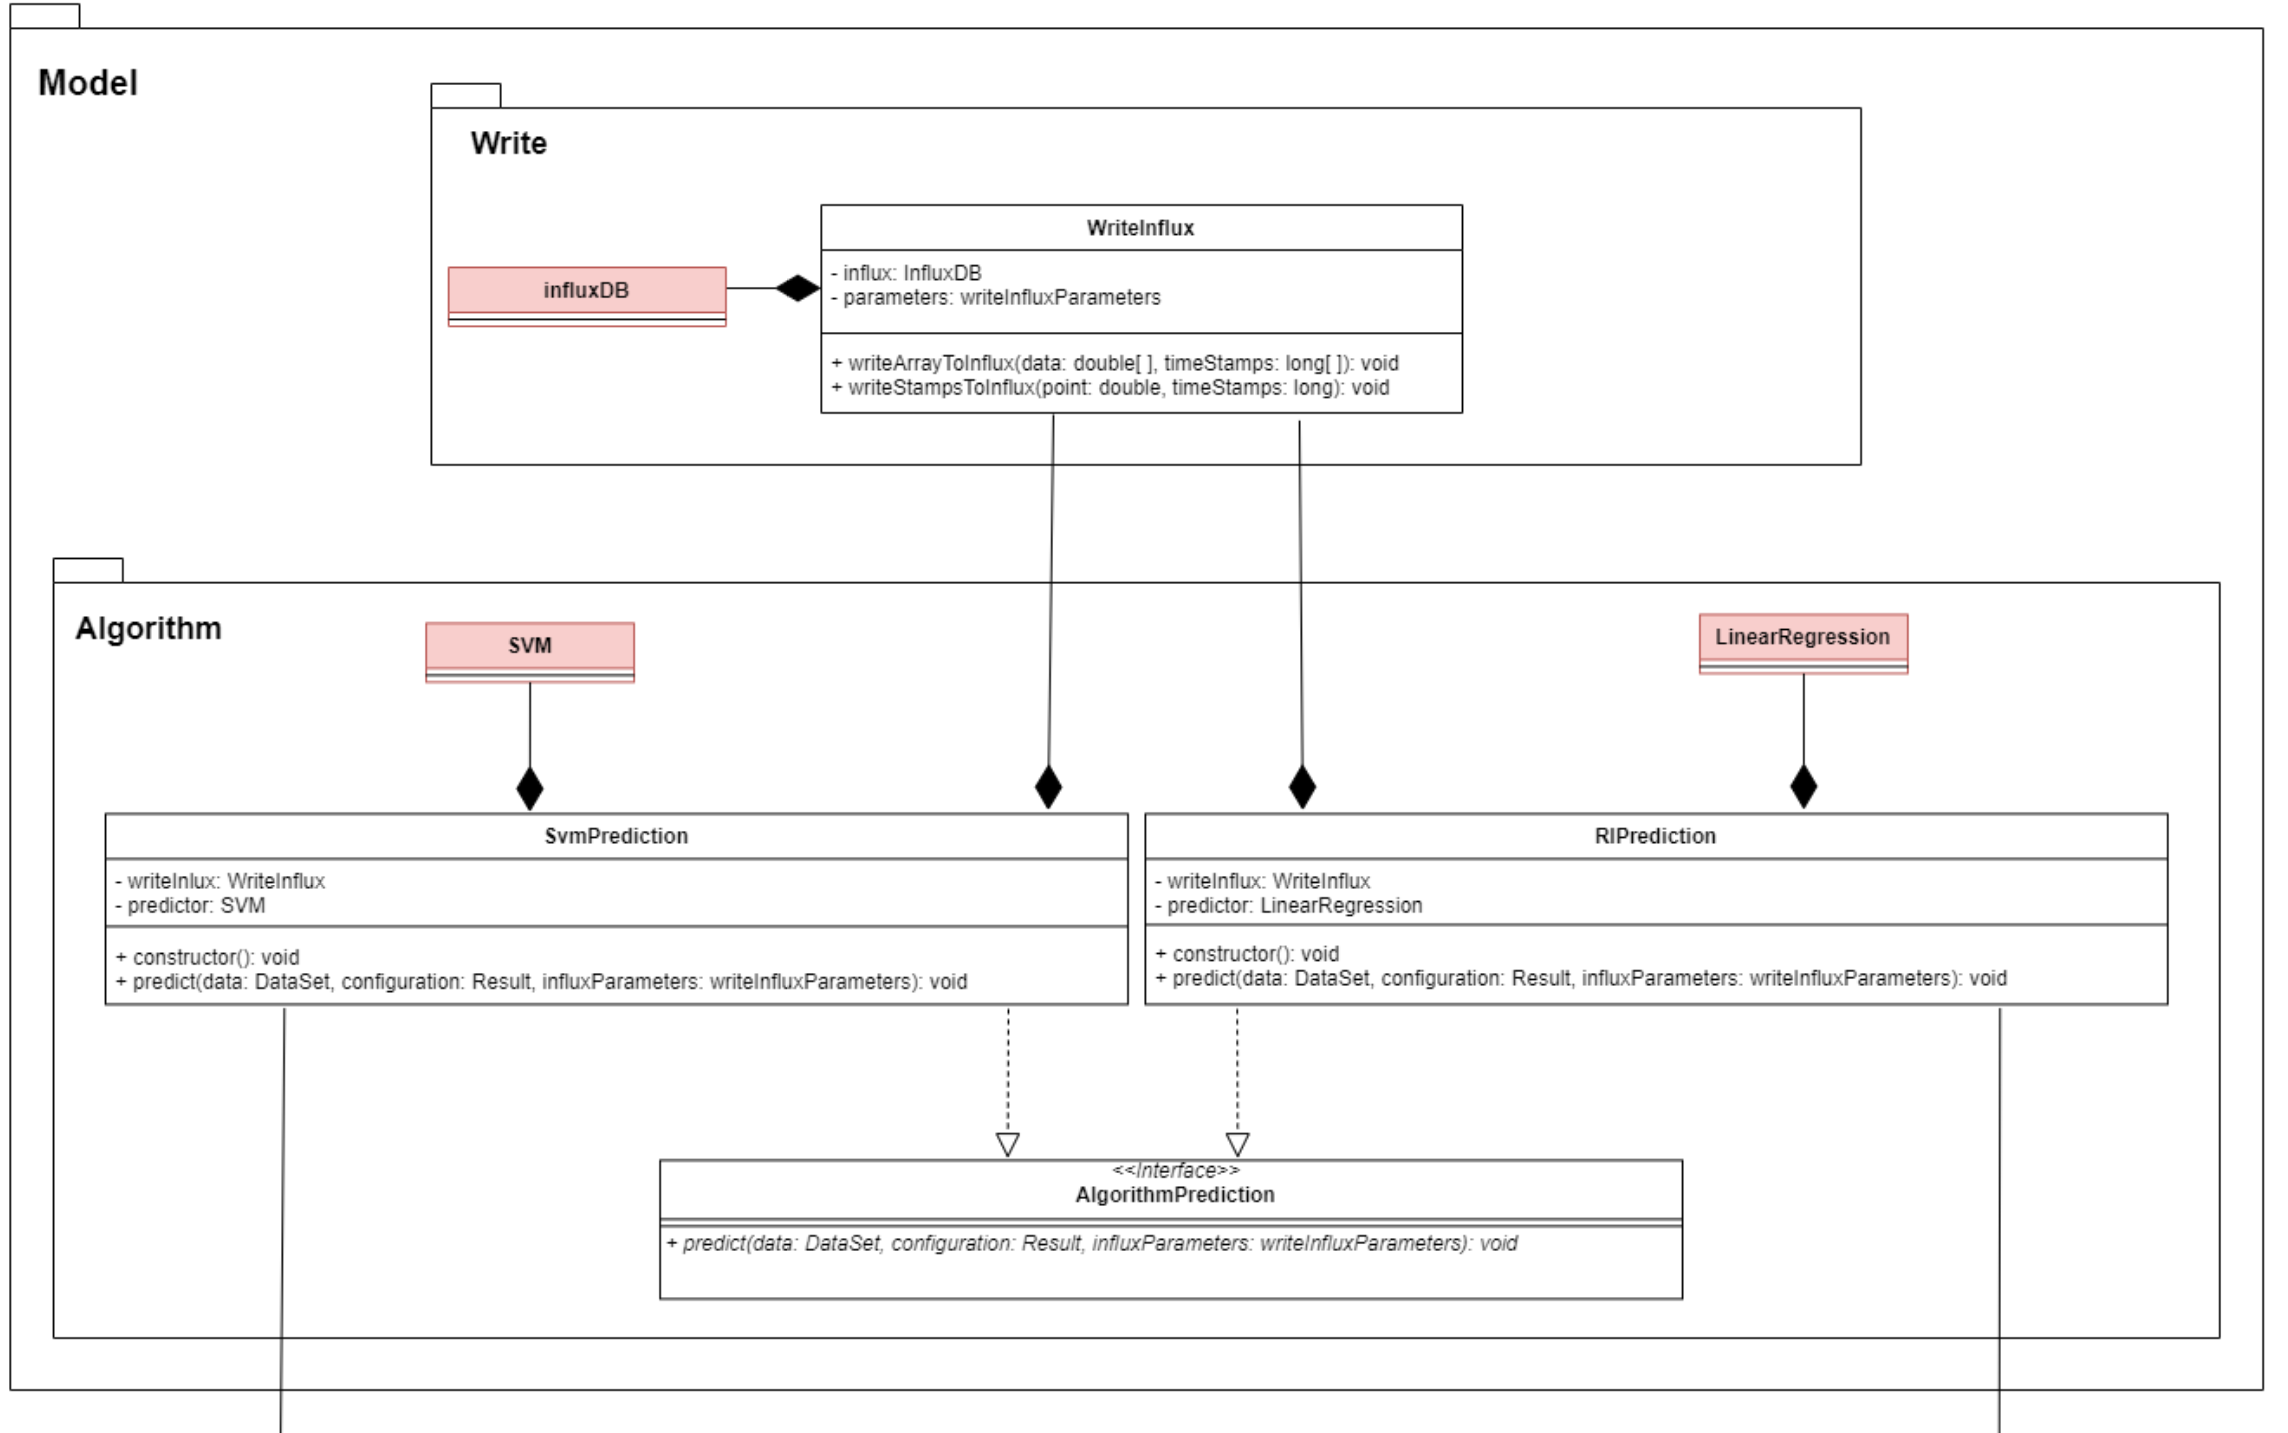
\includegraphics[width=\linewidth]{./img/Diagrammi/model-plug-in.png}
			\caption{Diagramma delle classi del Model}
		\end{figure}
	\end{figure}
\end{landscape}

\paragraph{View} \mbox{}\\ [1mm]
All'interno della View abbiamo inserito la componente Panel rappresentata dalla classe \textit{PanelCtrl}. Essa rappresenta il nostro pannello principale dal quale gli utenti possono interagire con il plug-in.
Inoltre attraverso la classe \textit{SelectInfluxDBCtrl} permettiao la selezione dalla datasource Grafana\glosp di tipo Influx su cui scrivere i risultati delle predizioni. In questo modo, sfruttiamo il meccanismo di Grafana\glosp che, dalla scrittura dei dati sul database di tipo Influx, permette l'aggiornamento continuo della View.
\paragraph*{PanelCtrl} \mbox{}\\ [1mm]
La classe che gestisce il pannello di controllo della nostra View è \textit{PanelCtrl} che estende la classe \textit{MetricsPanelCtrl} di Grafana\glo. \\
I campi dati di cui è necessaria una descrizione sono i seguenti:
\begin{itemize}
	\item nodeMap: contiene la mappatura dei predittori da fornire per la configurazione degli algoritmi;
	\item databaseParameters: è un oggetto di tipo WriteInfluxParameters e rappresenta quindi i parametri di configurazione del database ricevuti in input dall'utente;
	\item plotlyPanelUtil: è un oggetto di tipo PlotlyPanelUtil e rappresenta quindi un'istanza di tale classe importata dalla libreria Plotly per la realizzazione di un grafico personalizzato;
	\item processData: è un oggetto di tipo ProcessData e rappresenta quindi il legame tra View e Controller.
\end{itemize}
I metodi di cui è necessaria una descrizione sono i seguenti:
\begin{itemize}
	\item onDataReceived(Datalist): permette di ricevere i dati da Grafana\glosp e di realizzare delle operazioni. In particolare riceve i dati da InfluxDB e permette l'aggiornamento continuo dal Model;
	\item updateNodeMap(): permette l'aggiornamento della configurazione dei predittori e quindi della configurazione degli algoritmi;
	\item uploadButtonClick(): permette il caricamento del file JSON di configurazione ottenuto dall'applicativo di addestramento degli algoritmi di predizione;
	\item onInitEditMode(): permette la gestione della configurazione del pannello al momento della sua istanziazione da parte di Grafana\glo.
\end{itemize}
Gli altri metodi e campi dati presenti sono documentati dal loro stesso nome.
\paragraph*{SelectInfluxDBController} \mbox{}\\ [1mm]
La classe che gestisce il pannello di inserimento dei dati per la scrittura su InfluxDB, contenuto nel pannello di controllo, è SelectInfluxDBController.
Contiene un campo dati di tipo Datasource[] che rappresenta i parametri di ogni sorgente dati presente in Grafana\glo, su cui è possibile applicare le predizioni o scrivere i risultati ottenuti. Espone infine i due metodi per popolare ed interfacciarsi con tale parametri:
\begin{itemize}
	\item getDatasources(): permette di popolare l'array di Datasource effettuando una richiesta HTTP alle API\glosp di Grafana\glo;
	\item updateDatabaseParams(): permette di inviare al controller i dati inseriti dall'utente tramite la vista.
\end{itemize}
\paragraph*{Datasource} \mbox{}\\ [1mm]
È un tipo di dato che descrive i parametri di una sorgente di dati collegata a Grafana\glosp attraverso dei campi dati.
\paragraph*{Result}
\textit{Result} è un'interfaccia utilizzata per i risultati degli algoritmi di predizione. Definisce quindi un contratto che tutte le classi concrete, rappresentanti un nuovo algoritmo di predizione, dovranno rispettare e consiste nel metodo \textit{toStringJson()}. Esso ritorna un oggetto JSON in formato stringa che dovrà contenere tutti i dati caratteristici dell'algoritmo di addestramento.
\paragraph*{ResultSvm} \mbox{}\\ [1mm]
\textit{ResultSvm} è una classe concreta che implementa l'interfaccia \textit{Result} e descrive il risultato di un'algoritmo SVM\glosp lineare.
\paragraph*{ResultRl} \mbox{}\\ [1mm]
\textit{ResultRl} è una classe concreta che implementa l'interfaccia \textit{Result} e descrive il risultato di un'algoritmo Regressione lineare\glo.
\mbox{}
\begin{landscape}
	\begin{figure}
		\begin{figure} [H]
			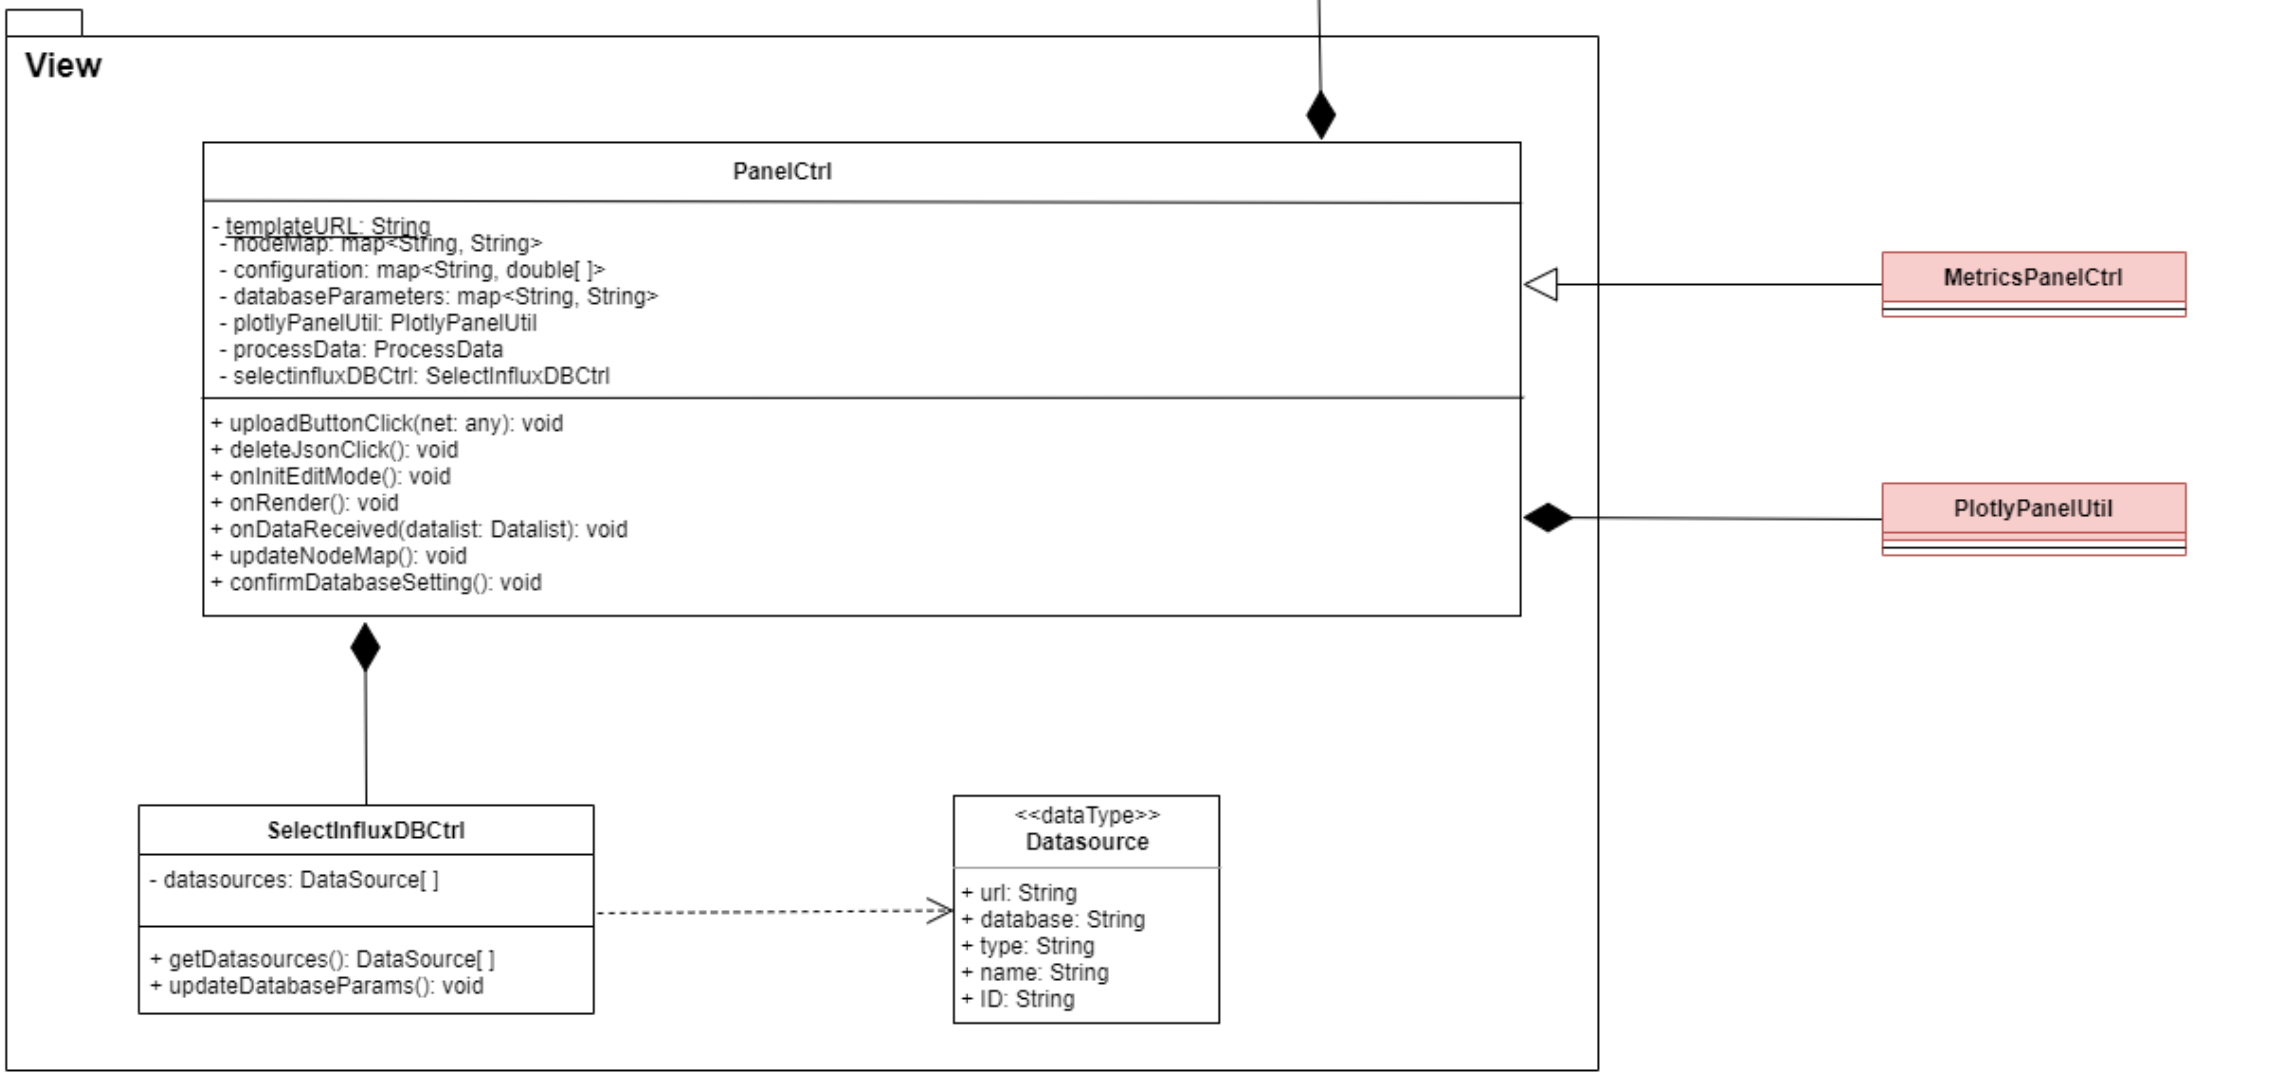
\includegraphics[width=\linewidth]{./img/Diagrammi/view-plug-in.png}
			\caption{Diagramma delle classi della View}
		\end{figure}
	\end{figure}
\end{landscape}

\paragraph{Controller} \mbox{}\\ [1mm]
All'interno del Controller viene implementata la trasformazione dei dati ricevuti dalla View, che rappresentano le interazioni dell'utente con il nostro pannello ed i flussi di dati ottenuti da Grafana\glo, ad azioni da eseguire sul Model.
Abbiamo deciso di implementare un design pattern\glosp strategy ottenendo la seguente struttura:
\begin{itemize}
	\item \textbf{ProcessData}: classe concreta che rappresenta il context del nostro strategy ed ha una dipendenza di tipo aggregazione con l'interfaccia \textit{PerformPrediction};
	\item \textbf{PerformPrediction}: interfaccia che rappresenta la strategia astratta;
	\item \textbf{ProcessSvm}: classe concreta che implementa \textit{PerformPrediction} e processa i dati per l'algoritmo Svm\glosp lineare;
	\item \textbf{ProcessRl}: classe concreta che implementa \textit{PerformPrediction} e processa i dati per l'algoritmo Regressione lineare\glo.
\end{itemize}

\paragraph*{ProcessData} \mbox{}\\ [1mm]
La classe concreta che rappresenta il context del nostro strategy è \textit{ProcessData}. Al suo interno viene scelto quale algoritmo di predizione processare sulla base dei dati e delle richieste ricevute. Inoltre ha una dipendenza di tipo aggregazione con l'interfaccia \textit{PerformPrediction}. \\
Il campo dati che necessita di una descrizione è \textit{nodeMap} che rappresenta la mappatura dei predittori. Gli altri campi dati, oltre a tutti i metodi, sono documentati dal loro stesso nome.
\paragraph*{PerformPrediction} \mbox{}\\ [1mm]
L'interfaccia che rappresenta la strategia astratta è \textit{PerformPrediction}. Essa definisce il contratto da rispettare per poter implementare una nuova classe concreta che processa i dati da fornire ad un algoritmo di predizione attraverso il metodo \textit{performPrediction(DataSet, Result, WriteInfluxParameters)}.
\paragraph*{ProcessSvm} \mbox{}\\ [1mm]
La classe concreta che implementa \textit{PerformPrediction} e rappresenta il componente che processa e trasforma i dati da fornire all'algoritmo Svm\glosp è \textit{ProcessSvm}.
Contiene il campo dati di tipo SvmPrediction che rappresenta la classe che implementa l'algoritmo di predizione all'interno del Model. Esso viene instanziato all'interno del costruttore assieme al binding dei metodi.
Infine all'interno del metodo \textit{performPrediction(DataSet, Result, WriteInfluxParameters)} viene richiamata la predizione dell'algoritmo.
\paragraph*{ProcessRl} \mbox{}\\ [1mm]
La classe concreta che implementa \textit{PerformPrediction} e rappresenta il componente che processa e trasforma i dati da fornire all'algoritmo regressione lineare\glosp è \textit{ProcessRl}.
Contiene il campo dati di tipo RlPrediction che rappresenta la classe che implementa l'algoritmo di predizione all'interno del Model. Esso viene instanziato all'interno del costruttore assieme al binding dei metodi.
Infine all'interno del metodo \textit{performPrediction(DataSet, Result, WriteInfluxParameters)} viene richiamata la predizione dell'algoritmo.
\paragraph*{WriteInfluxParameters} \mbox{}\\ [1mm]
È un tipo di dato che descrive i parametri necessari alla connessione e alla scrittura in un database Influx.
\paragraph*{Datalist} \mbox{}\\ [1mm]
È una classe che descrive le serie numeriche ottenute da Grafana\glo. Contiene al suo interno il nome della serie ed un array di coppie di punti formati da timestamp e valore.
\paragraph*{DataSet} \mbox{}\\ [1mm]
È una classe che descrive le serie numeriche elaborate e pronte per essere inviate agli algoritmi di predizione. Contiene al suo interno una array di serie numeriche e ed un array di timestamp relativi ai singoli punti delle serie numeriche.
\mbox{}
\begin{landscape}
	\begin{figure}
		\begin{figure} [H]
			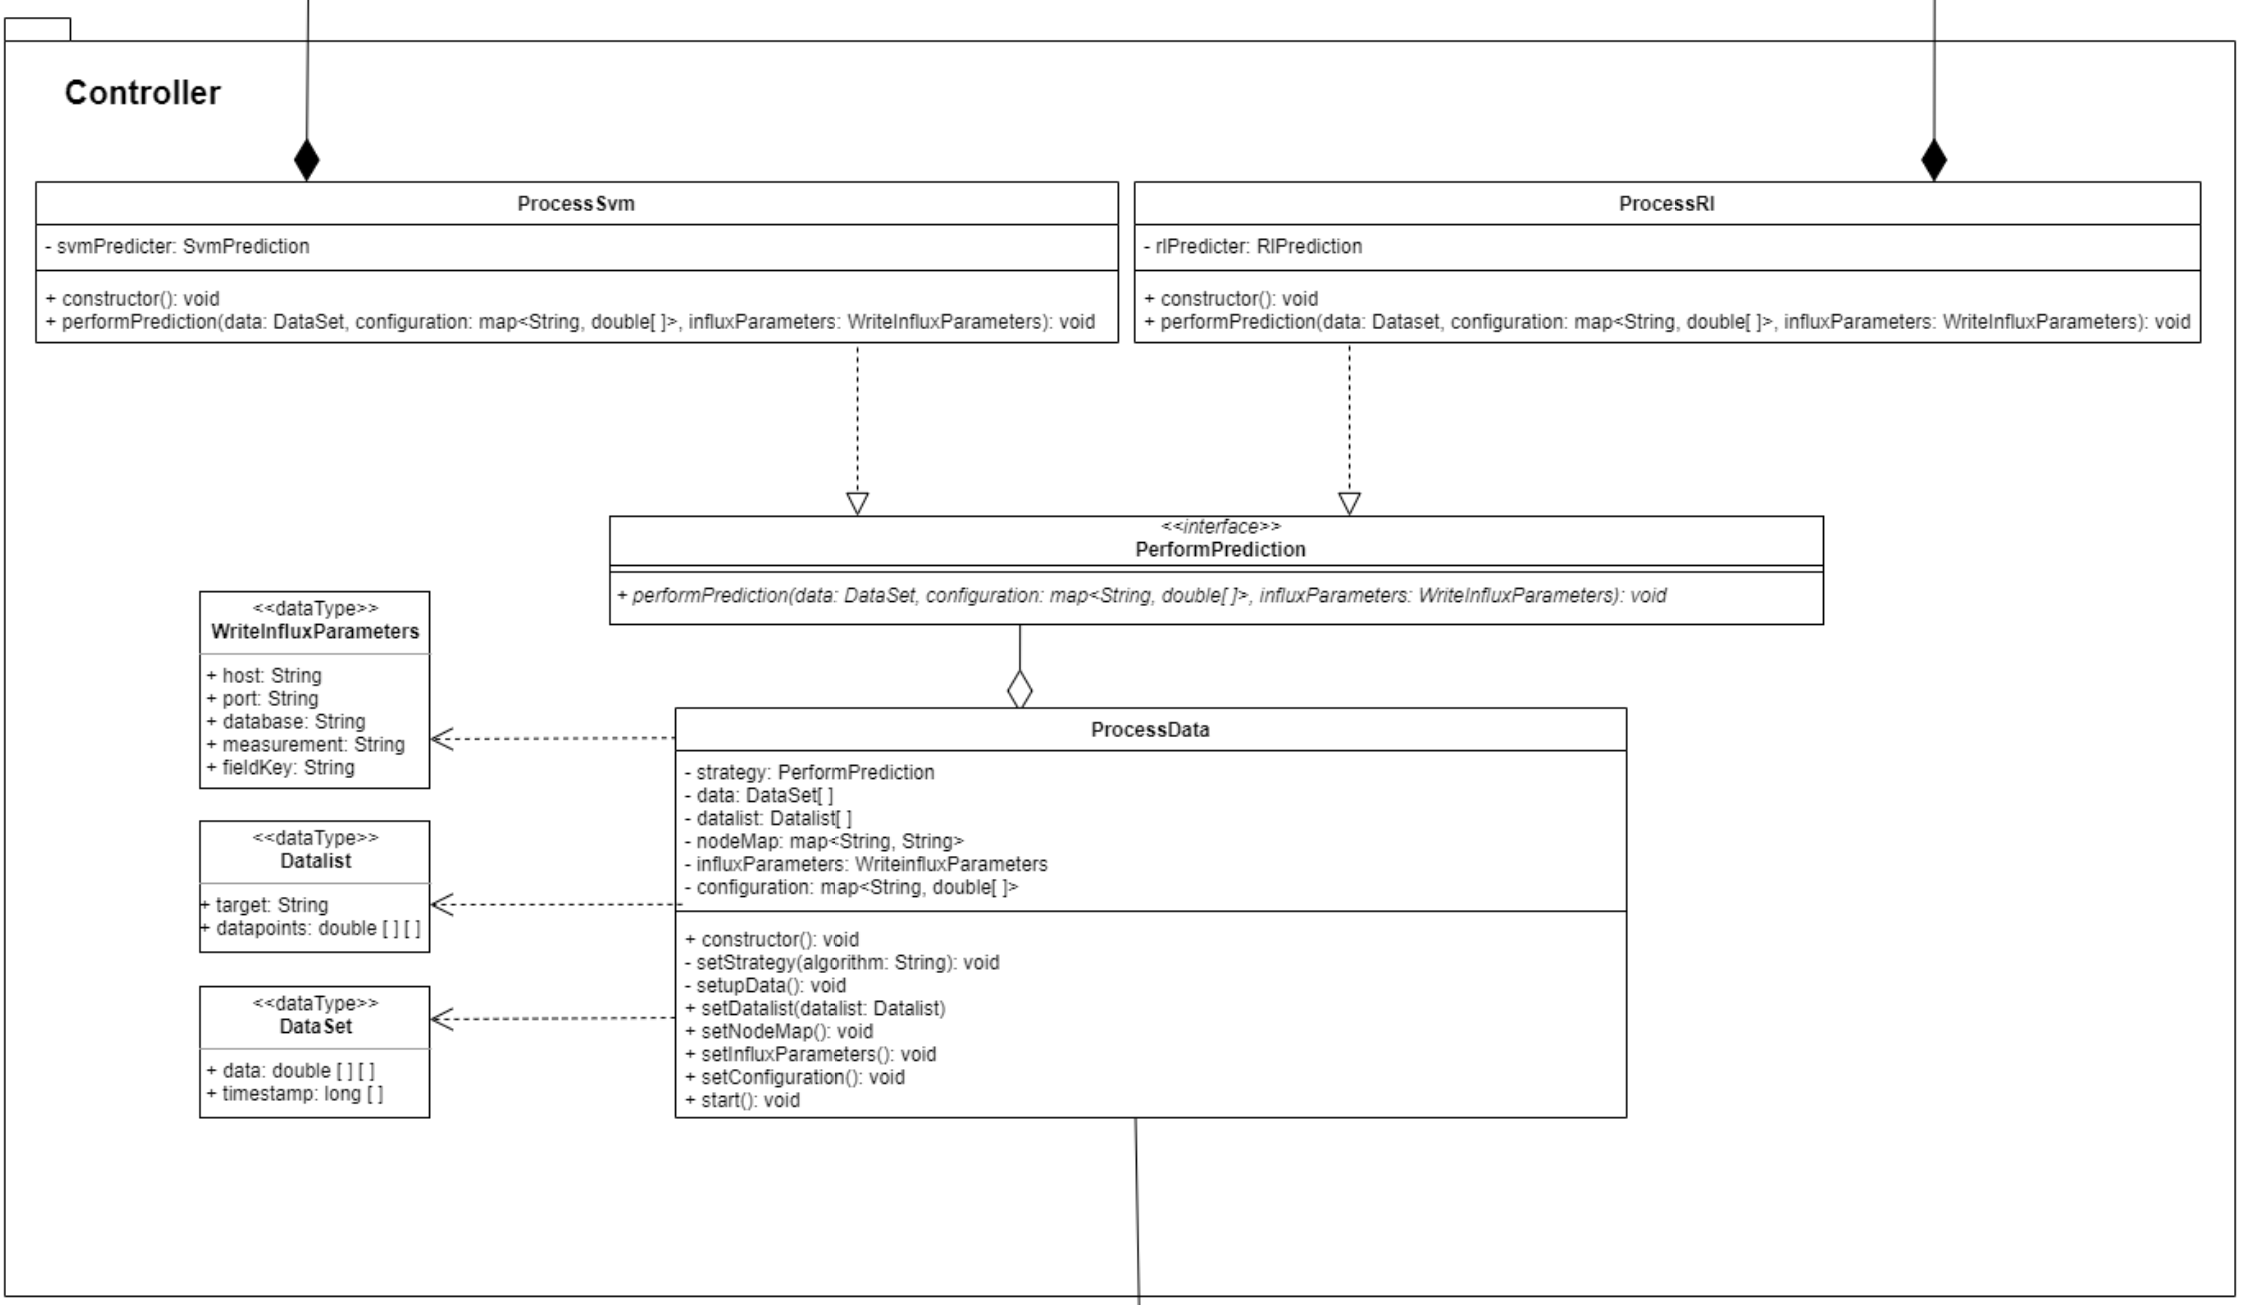
\includegraphics[width=\linewidth]{./img/Diagrammi/controller-plug-in.png}
			\caption{Diagramma delle classi del Controller}
		\end{figure}
	\end{figure}
\end{landscape}
\paragraph*{Diagramma di sequenza} \mbox{}\\ [1mm]
Per spiegare meglio l'insieme di azioni compiute al fine di processare i dati per eseguire la predizione degli algoritmi, illustriamo un diagramma di sequenza che prende in esame SVM\glo. Il procedimento è indicativo anche per gli altri algoritmi ed è auto documentato dal diagramma stesso.
\mbox{}
\begin{landscape}
	\begin{figure}
		\begin{figure} [H]
			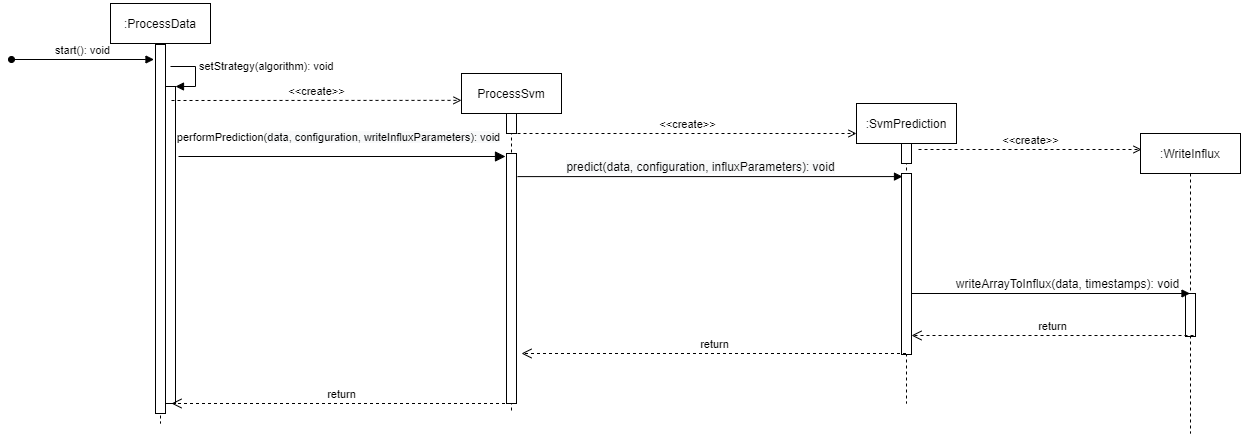
\includegraphics[width=\linewidth]{./img/Diagrammi/ds-plug-in.png}
			\caption{Diagramma di sequenza di processo dei dati per SVM}
		\end{figure}
	\end{figure}
\end{landscape}
